\chapter{The Large Hadron Collider}

The Large Hadron Collider (LHC) is a circular proton-proton collider, 27 km in circumference and between 40 and 175 m below the surface, located at the European Organization for Nuclear Research (CERN) on the French-Swiss border near the city of Geneva.
Designed to collide protons at a maximum center-of-mass energy $\sqrt{s} = 14\TeV$, the LHC has delivered collisions at $\sqrt{s} = 7, 8 \TeV$ during Run 1 (2010-2012) and at $\sqrt{s} = 13\TeV$ during Run 2 (2015-2018).
While the LHC is primarily a proton-proton collider, lead (Pb) ion beams of energy of up to 2.8 TeV per nucleon are used to produce lead-lead and proton-lead collisions.
In this thesis, we focus exclusively on data recorded from proton-proton collisions during Run 2.

\begin{figure}[htbp]
  \centering
  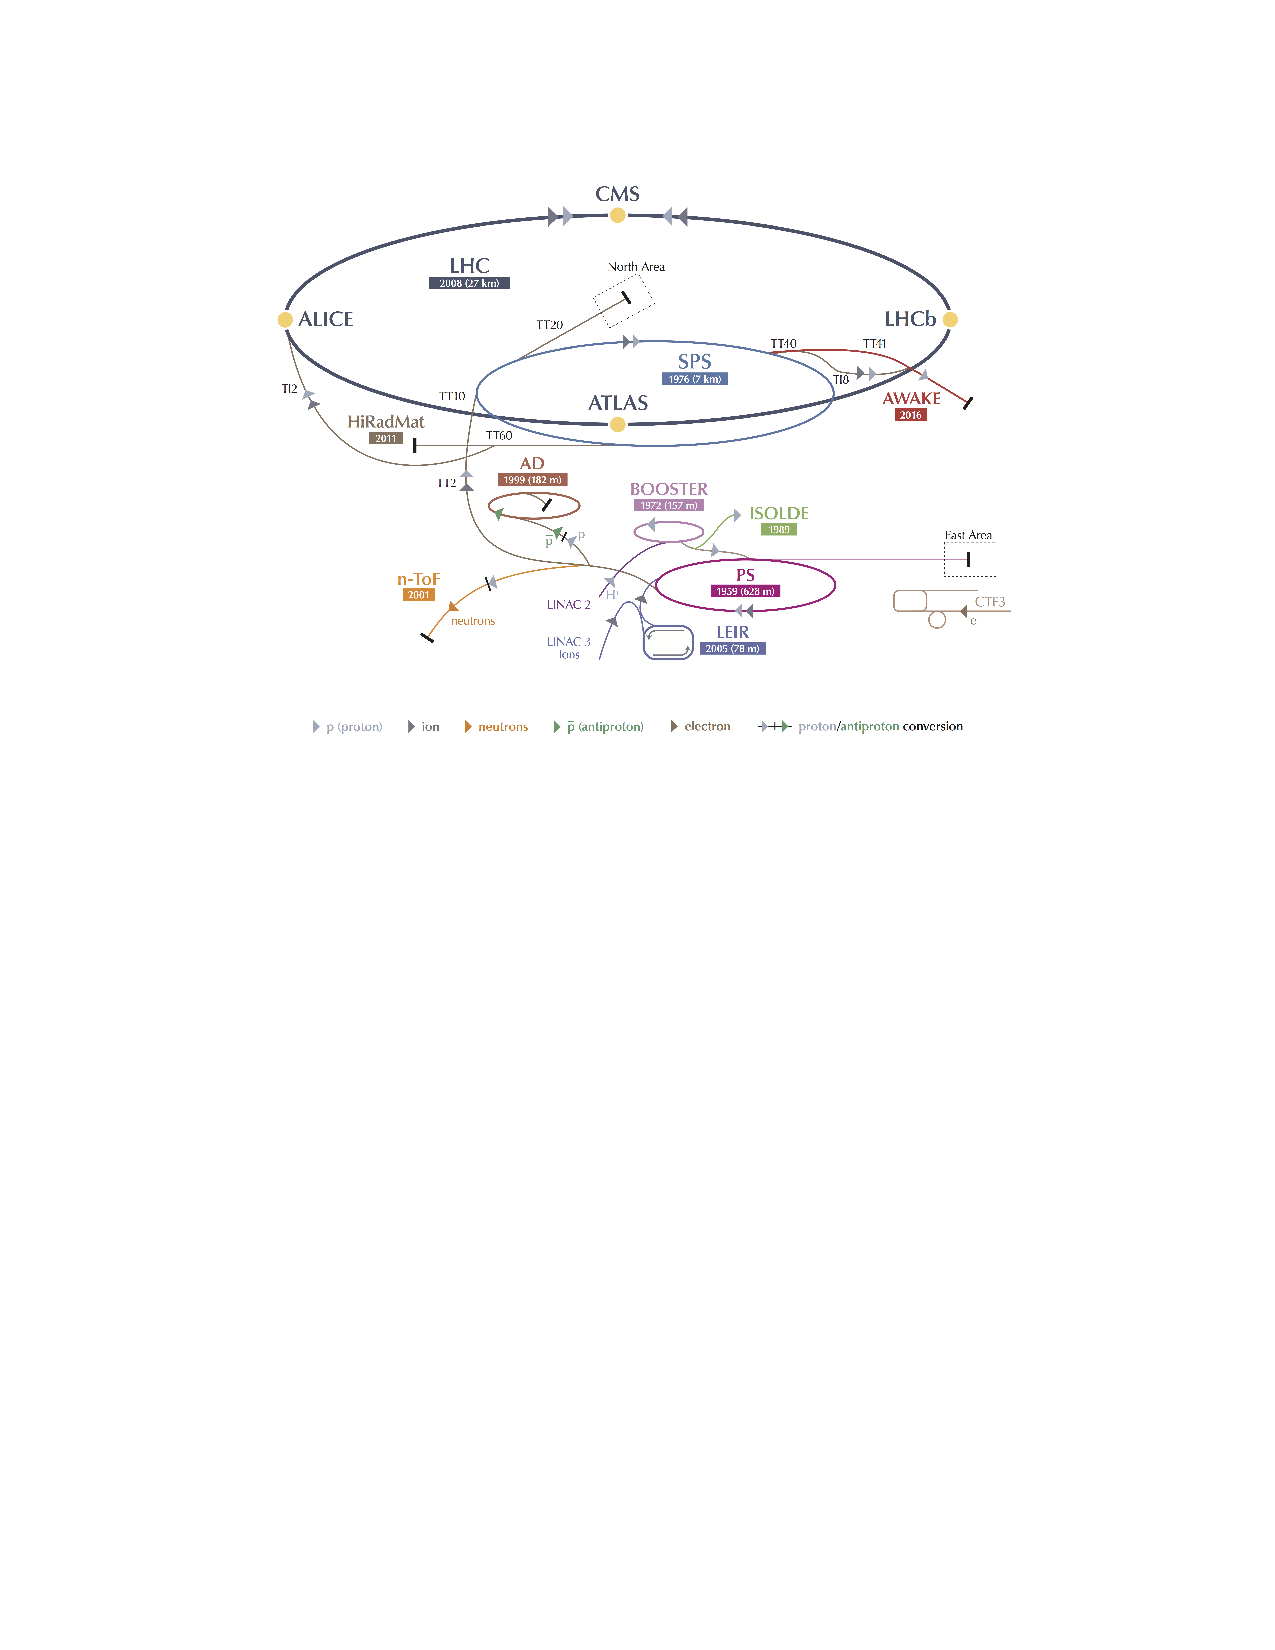
\includegraphics[width=0.625\textwidth]{Collider/Figures/LHC_diagram.pdf}
  \caption{
    A schematic representation of the CERN accelerator complex. 
    The LHC (dark blue) is fed protons by a chain of intermediate accelerators, beginning with LINAC2 (light pink).
    Reprinted from the CERN Document Server~\cite{}. % https://cds.cern.ch/record/2636343?ln=en
  }
  \label{fig:lhc}
\end{figure}

The LHC is the final stage of the CERN accelerator complex depicted in Figure~\ref{fig:lhc}.
Hydrogen atoms are stripped of their electrons and accelerated to an energy of 50\GeV by the LINAC2 linear acceleration.
Following this, they are injected into the Booster ring, the Proton Synchrotron (PS), and the Super Proton Synchrotron (SPS) and accelerated to 1.4, 26, and 450\GeV, respectively.
After the SPS, the protons are injected into the two counter-circulating rings of the LHC in up to 2808 discrete bunches with a bunch spacing of 25\ns.
The two beams intersect in eight places along the LHC with detector experiments CMS, ATLAS, LHCb, and ALICE each located at an intersection point.

The LHC is a synchrotron containing 1232 superconducting NbTi dipole magnets measuring 15 m in length, each with a peak dipole field of 8.33 Tesla. 
There are an additional 492 quadrupole magnets measuring 5-7 m in length which focus the beams in between the dipole magnets.
Due to space limitations in the tunnels, the beam pipes are magnetically coupled and the magnets share the same superfluid liquid helium cryostatic system to achieve the 1.9K temperature required to achieve the desired magnetic field strength.

The number of events produced at the LHC is given by
\begin{equation}
  N(pp \rightarrow X) = \int dt L(t) \sigma(pp \rightarrow X),
\end{equation}
where $\sigma$ is the cross section of the process and $L$ is the instantaneous luminosity of the machine given by
\begin{equation}
  L = \frac{N_b^2 n_b f_{\text{rev}} \gamma}{4 \pi \epsilon \beta^*} \times F,
\end{equation}
where $N_b$ is the number of particles per bunch ($\mathcal{O}(10^11)$),
$n_b$ is the number of bunches per beam,
$f_{\text{rev}}$ is frequency of revolution,
$\gamma$ is the Lorentz factor of the beam,
$\epsilon$ is transverse emittance of the beam,
$\beta^*$ is beta function of the beam at the collision point,
and $F$ is the geometric luminosity reduction factor due to the crossing angle at the interaction point.
The instantaneous luminosity decreases exponentially as a function of time due to $N_b$ and $n_b$ being reduced by collisions.
The LHC is designed to deliver an initial instantaneous luminosity of $\mathcal{O}(10^{34}) \percms$.

As all known cross sections are time-independent, the total number of events is directly proportional to the integrated luminosity given by
\begin{equation}
  L_{\text{int}} = \int_0^T dt L(t) = L(0) \tau_L \left(1 - e^{-\sfrac{T}{\tau_L}} \right),
\end{equation}
where $T$ is the time since starting collisions,
$L(0)$ is the initial instantaneous luminosity,
and $\tau_L \approx 15$ the characteristic beam loss timescale for the LHC.
The total luminosity delivered by the LHC and recorded by CMS during the 2016 is shown in Figure~\ref{fig:lumi}.

\begin{figure}[htbp]
  \centering
  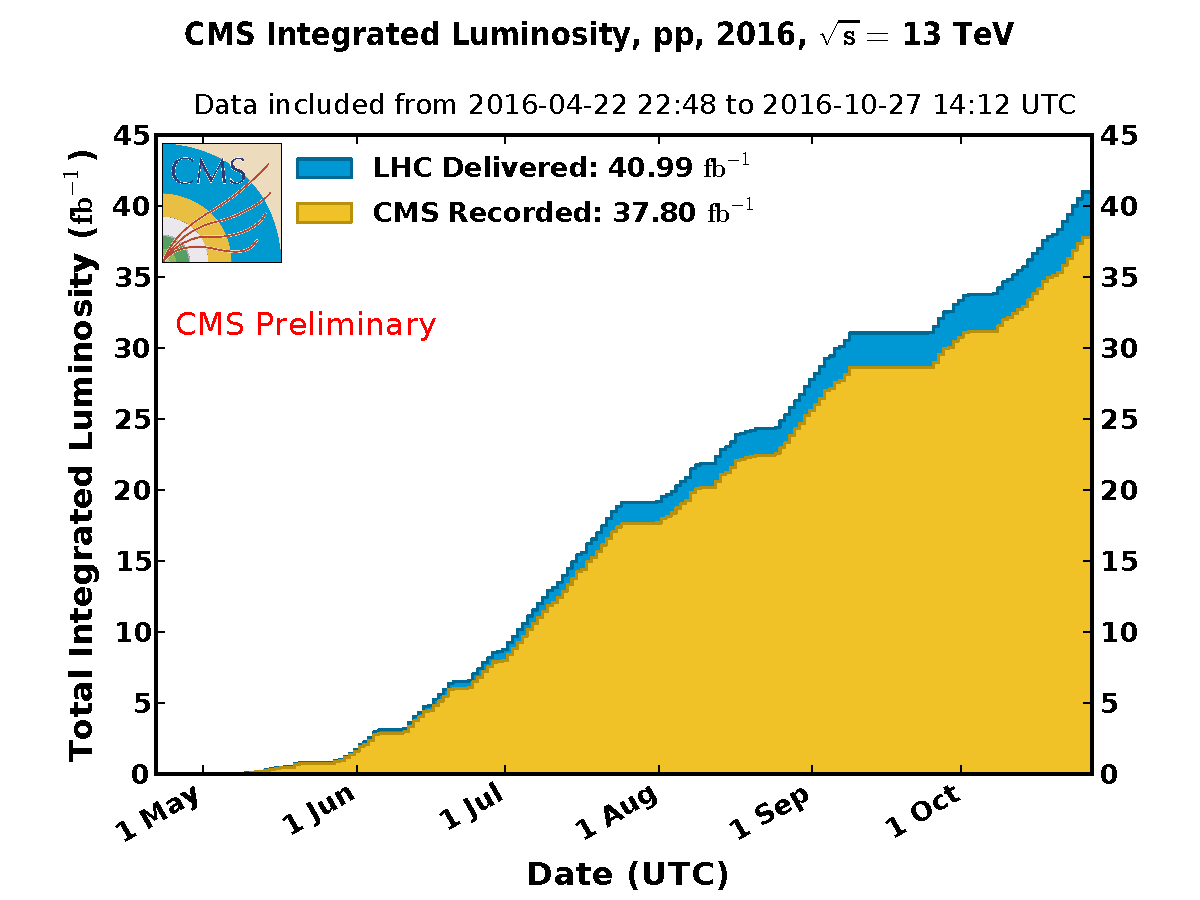
\includegraphics[width=0.75\textwidth]{Collider/Figures/lumi_2016.pdf}
  \caption{
    The total integrated luminosity of the LHC during proton-proton collisions during 2016.\cite{}
    While a total luminosity of 41\fbinv was collected, only a subset during which the detector operated optimally is used in this thesis. This corresponds to 36\fbinv of data.
    % https://twiki.cern.ch/twiki/bin/view/CMSPublic/LumiPublicResults
  }
  \label{fig:lumi}
\end{figure}

\section{Collider Phenomenology}

The proton is a composite particle consisting of valence quarks, sea quarks, and gluons, collectively referred to as partons.
When colliding protons at the LHC, we are actually interested in the inelastic scattering of a pair of partons from the incident protons.
Each parton $a,b$ carries a fraction of the momentum of the incoming proton $x_{a,b}$ following the particle-dependent parton distribution functions (PDFs) $f_{a,b}$.
The differential cross section for $2\rightarrow N$ parton scattering process is given by
\begin{equation}
  \text{d}\sigma \left(ab \rightarrow \{c_i\} \right) =
  \frac{(2\pi)^4}{2s} \left( \prod_i \frac{\text{d}^3 p_i}{(2\pi)^3} \right)
  \cdot \delta^4 \left(k_a + k_b - \sum_i p_i \right)
  \cdot \abs{ \mathcal{M} \left(ab \rightarrow \{c_i\} \right)}^2
\end{equation}
where $k_{a,b} = x_{a,b} \sqrt{s}$ are the momenta of the incoming partons, $\{p_i\}$ are the momenta of the outgoing partons $\{c_i\}$, and $\mathcal{M}$ is the matrix element of the process.

This parton level scattering, called the hard scattering process, is perturbatively calculable through standard QFT methods.
However, the hard scattering does not include any effects related to the PDFs of the incoming partons or the decay and hadronization of the outgoing partons into the final state particles (called the parton shower), both of which involve non-pertubative aspects of QCD.
Fortunately, the collinear factorization theorem states that the probability of obtaining the final state $X(\Theta)$ from a hadron collision can be calculated as the product of the probability that specific partons $a,b$ are involved in the interaction, the probability for the hard scattering to produce outgoing partons $\{c_i\}$, and the formation of final state hadrons from these outgoing partons.
The factorization process is not unique and requires the choice of an arbitrary energy scale $\mu_F$, which defines a lower bound for interactions to be considered part of the hard scattering.  

Including the effects from PDFs and parton showering (PS), the general cross section for $pp \rightarrow X(\Theta)$ is
\begin{align}
  \label{eqn:ppx}
  \frac{\text{d}\sigma}{\text{d}\Theta} \Big(pp \rightarrow X(\Theta) \Big) =
  \sum_{a,b} \int & \text{d} x_a f_a(x_a, \mu_F) \cdot \text{d} x_b f_b(x_b, \mu_F)  \nonumber \\
  & \times \text{d}\sigma \left(ab \rightarrow \{c_i\} \right)
  \times D \left( \{c_i\} \rightarrow X(\Theta) \right) 
\end{align}
where the sum is over the initial state partons and $D$ is the fragmentation function that describes parton shower process resulting in the observed final state.
The following sections discuss the simulation of the three main elements of Equation~\ref{eqn:ppx}: the parton distribution functions $f_a$, the hard scattering cross section $\text{d}\sigma$, and the fragmentation function $D$.

\subsection{Parton Distribution Functions}

\subsection{Hard Scattering}

\subsection{Parton Shower}
